\section{Durchführung}
%% \subsection{Übersicht}
Es finden insgesamt drei Versuchsteile statt.

%auskommentiert, da in andere abschnitte reinkopiert

\subsection{Die Zeitkonstante des RC-Gliedes}
\label{sec:durchf_a}
Im ersten Veruchsteil soll die Zeitkonstante $\tau$ eines RC-Gliedes bestimmt werden.
Hierzu wird der Entladevorgang des Kondensators bei angelegter Rechteckspannung untersucht.
Die entsprechende Schaltung mitsamt Oszilloskop ist in Abbildung \ref{fig:zeitkonst} zu sehen.
\begin{figure}[H]
    \centering
    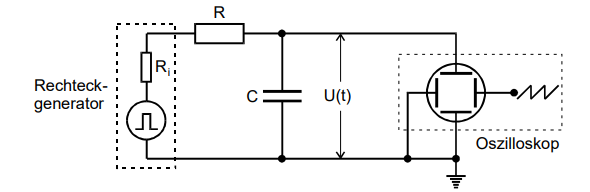
\includegraphics[height=5cm]{abbildungen/zeitkonstante.png}
    \caption[short]{Schaltung zur Bestimmung der Zeitkonstanten \cite{man:v353}.}
    \label{fig:zeitkonst}
\end{figure}
\noindent
% Anmerkung: Die gemessene Rechteckspannung ist zwischen + und - hin und hergesprungen -- kann och auch noch in der Auswertung erwähnen.
Der Entladeprozess beginnt, sobald die Rechteckspannung auf Null zurück gesprungen ist, und dauert so lange, wie sie auf Null verharrt\footnote{Ganz 
analog kann zur Bestimmung von $\tau$ auch der Aufladevorgang untersucht werden.
Dieser beginnt beim Sprung der Generatorspannung von Null auf den Maximalwert und dauert so lange, 
wie sie auf diesem Wert verbleibt.}.
Somit werden stets Ausschnitte des eigentlich unendlich langen Vorgangs beobachtet.
Für eine höhere Ablesegenauigkeit werden Rechteckfrequenz $f$ und Ablenkgeschwindigkeit des Kathodenstrahls so eingestellt, 
dass ein ganzer Abschnitt möglichst groß auf dem Oszilloskop zu erkennen ist.
Dabei muss auch die Position des Spannungsnullpunktes bekannt sein.
Diese kann ermittelt werden, indem eine gegen $\tau$ große Frequenz $f$ eingestellt wird, da $U_\text{C}$ somit praktisch auf Null sinkt.
Eine geeignete Darstellung am Oszilloskop ist in Abbildung \ref{fig:spannungsverlauf} einzusehen.
% Die Zeitachseneichung kann am Drehknopf für die Ablenkgeschwindigkeit abgelesen werden.
% Außerdem ist wichtig, dass der Triggerpegel richtig eingestellt ist.
\begin{figure}[H]
    \centering
    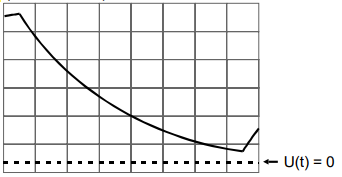
\includegraphics[height=4cm]{abbildungen/geeignete_darstellung.png}
    \caption{Geeignete Darstellung des Spannungsverlaufs am Kondensator \cite{man:v353}.}
    \label{fig:spannungsverlauf}
\end{figure}
\noindent
Für die hier protokollierte Messreihe wird die Rechteckfrequenz auf $f = \qty{30.7}{\hertz}$ gestellt.
Das Triggersignal wird DC gekoppelt.
Die Pegel Voltdiv und Timdiv werden so eingestellt, 
dass auf der vertikalen Achse ein Kästchen \qty[]{0.2}{\volt} und auf der horizontalen Achse \qty{2}{\ms} entspricht.
Mit dem Regler zum Anpassen der x-Position wird die Kurve so verschoben, 
dass in Abhängigkeit von der verschobenen Zeit die Spannung an der y-Achse schrittweise abgelesen und notiert werden kann.
% a)
% Rechteckspannung +- amplitude 
% Entladungskurve auf Oszilloskop wird schrittweise abgelesen und notiert

\subsection{Die Amplitude und Phasenverschiebung der Kondensatorspannung}
Im zweiten Teil des Versuchs wird die Amplitude $A$ der Kondensatorspannung und die Phasenverschiebung $\phi$ zwischen Generator-
und Kondensatorspannung eines RC-Gliedes bei angeschlossener Sinusspannung in Abhängigkeit der Frequenz untersucht.
Hierfür wird ein Zweikanal-Oszillograph wie er in Abbildung \ref{fig:ampl_phasenverschiebung} zu sehen ist angeschlossen.
Das Triggersignal beider Kanäle wird AC gekoppelt.
Der Kondensator wird an Kanal 1 und der Generator an Kanal 2 angeschlossen.
\begin{figure}[H]
    \centering
    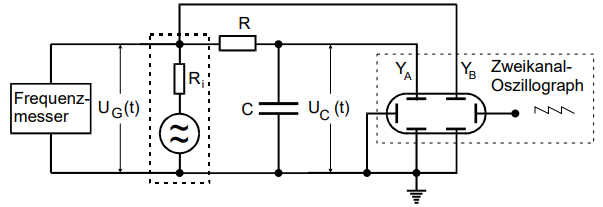
\includegraphics[height=5cm]{abbildungen/ampl_phasenverschiebung.png}
    \caption{Schaltung zur Messung der Amplitude und Phasenverschiebung \cite{man:v353}.}
    \label{fig:ampl_phasenverschiebung}
\end{figure}
\noindent
Es werden mehrere Frequenzen $\omega$ zwischen ca. \qty{0}{\hertz} und \qty{1000}{\hertz} eingestellt.
Dabei müssen je nach Größenordnung die Regler Timediv und Voltdiv angepasst werden.
Zum leichteren Ablesen der einzelnen Werte können die Graphen erneut mittels des x-Positionsreglers verschoben werden.
Generell ist darauf zu achten, dass beide Graphen symmetrisch zur x-Achse liegen.
Am Oszilloskop ergibt sich in etwa ein Graph wie in Abbildung \ref{fig:graph_phasenverschiebung}.
\begin{figure}[H]
    \centering
    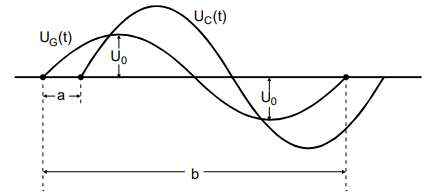
\includegraphics[height=3cm]{abbildungen/graph_phasenverschiebung.png}
    \caption{Darstellung zur Bestimmung von $\phi$ \cite{man:v353}.}
    \label{fig:graph_phasenverschiebung}
\end{figure}
\noindent
Es wird festgestellt, dass die Amplitude der Generatorspannung einen konstanten Wert $U_0 = \qty[]{1.55}{\volt}$ unabhänig von $\omega$ hat.
Die Amplitude der Kondensatorspannung $A$ kann sofort abgelesen werden.
Zur Bestimmung der Phasenverschiebung $\phi$ muss zunächst der zeitliche Abstand $a = \Delta t$ der beiden Nulldurchgänge bestimmt werden.
Die Schwingungsdauer $b$ lässt sich mittels $b = \frac{1}{\omega}$ ermitteln.
Somit ergibt sich 
\begin{align}
    \phi = 2 \pi \, \frac{a}{b}.
    \label{eq:phase}
\end{align}
%

\subsection{Der RC-Kreis als Integrator}